\documentclass[a4 paper]{report}
%\usepackage[firstpage]{draftwatermark} optional
%\SetWatermarkScale{1}

\usepackage{graphicx}
%\usepackage{bidi}
\usepackage[no-math]{fontspec}
\usepackage{xltxtra,url,amsmath}
\usepackage[quiet]{polyglossia}
\usepackage{amsmath,amsthm,amsfonts}
\usepackage{setspace}
\usepackage{paralist}
\usepackage[geometry]{ifsym}
\usepackage{float}
\usepackage{fancybox}	
\usepackage{calc}
\usepackage{xcolor}
\usepackage{hyperref}
	
\floatstyle{ruled}
\newfloat{program}{thp}{lop}
\floatname{program}{خوارزمية}
% Use the option [numerals=maghrib] to have the numbers printed in Arabic
\setdefaultlanguage[numerals=maghrib]{arabic} % Remove  [numerals=maghrib] if you don't want the numbers to be printed in Arabic

\setotherlanguage[variant=british]{english}
\setmainfont{AL-Mohanad}
\setromanfont{Junicode}
\defaultfontfeatures{Scale=MatchLowercase}
\setmonofont{AL-Mohanad}
\setsansfont{AL-Mohanad}
\newfontfamily\arabicfont[Script=Arabic,Scale=1]{Amiri}
\newfontfamily\arabicfonttt[Script=Arabic,Scale=1.3]{Times New Roman}
%\let\arabicfonttt\sfamily
\gappto\captionsarabic{\renewcommand{\chaptername}{الباب}}


\newcommand\words[1]{\expandafter\xwords\csname c@#1\endcsname}
\def\xwords#1{\ifcase#1\or
الأول\or
الثاني\or
الثالث\or
الرابع\or
الخامس\or
السادس\or
السابع\or
الثامن\or
التاسع\or
العاشر\or
\else
I need more words\fi}
%\usepackage{etoolbox}%% uncomment if 'etoolbox' isn't already being loaded
\makeatletter
\patchcmd{\@makechapterhead}{\thechapter}{\words{chapter}}{}{}
\parindent 0pt
\makeatother

\title{طباعة كتاب بإستخدام حزمة \\
\eng{Polyglossia}}
\author{د. فيصل بن عبدالله المالكي}
\date{\today}

%% Optional
\newtheoremstyle{mystyle}
{\topsep}
{\topsep}
{\upshape}
{}
{\bfseries}
{ :}
{\newline}
{

\rule[0.5\baselineskip]{0.5\textwidth}{1pt}%
\newline\fcolorbox{black}{gray!20}{%
\thmname{#1}\thmnumber{ \textup{#2}}\thmnote{ \textnormal{(#3)}}%
}
\medskip
}

% You can add as much as new classes you can

\theoremstyle{mystyle}
\newtheorem{theorem}{$\:\:\:\square $ \arabicfonttt{\underline{\large{نظرية}}}}[chapter]
\newtheorem{example}{$\square$ \arabicfonttt{\underline{مثال}}}[chapter]
\newtheorem{note}{\SquareShadowB\arabicfonttt {\underline{ ملاحظـة }}}[chapter]
\newtheorem{definition}{\SquareShadowB\arabicfonttt {\underline{ تعريف }}}[chapter]

\renewcommand\thetheorem{{\bf \arabic{theorem}.\arabic{section}}}
\renewcommand\theexample{{\bf \arabic{example}.\arabic{section}}}
\renewcommand\thedefinition{{\bf \arabic{definition}.\arabic{section}}}
\renewcommand\thenote{{\bf \arabic{note}.\arabic{section}}}

\newtheorem{excercise}{\SquareShadowB\arabicfonttt {\underline{ تمرين }}}[chapter]
\newtheoremstyle{Excercises}{12pt}{12pt}{\bfseries}%
{}{\rmfamily}{:}{\newline}{}
\theoremstyle{Excercises}
\newtheorem{Excercises}{\SquareShadowB\arabicfonttt {\underline{ تمارين }}}[chapter]
\renewcommand\theExcercises{{\bf \arabic{Excercises}.\arabic{section}}}

\renewcommand{\thechapter}{\arabic{chapter}}
\newcommand{\eng}{\textenglish}  % To insert English text
\addto\captionsarabic{\renewcommand{\bibname}{المراجع}}

%To control Page Dimension use the following commands
%\pdfpagewidth 12.25in
%\pdfpageheight 10.75in

\begin{document}
\maketitle
\tableofcontents
\doublespacing
\chapter{ مقدمة}

سوف نقدم في هذا الملف قالبا لكتابة كتاب بإستخدام حزمة 
\eng{Polyglossia}
في بيئة \eng{\LaTeX}، علما أنه يمكن تغيير مايلزم لإضافة أية تعديلات على الملف. ولضمان نجاح تجربة إستخدام الملف فيجب أن يكون لديك
\begin{enumerate}
  \item الإصدار الأخير من حزمة \eng{MikTex or TexLive}
  \item محرر يدعم الكتابة باللغة العربية مثل \eng{WinEdt 10.00 , TexWork}
  \item إجراء عملية التحويل \eng{Compiling} بإستخدام \eng{XeLatex}
  \item التأكد من وجود الخطوط أعلاه في جهاز الكمبيوتر لديك. و يمكن تحميل أي خطوط تود من خلال المواقع
  \setLR
  \begin{itemize}
    \item http://www.arfonts.net/
    \item https://fonts.google.com/
  \end{itemize}
  \setRL
  \item  في حال وجود أية ملاحظات، آمل التكرم بالتواصل معي على الإيميل
  \href{mailto:Faisal_malki1@hotmail.com}{Faisal\_malki1@hotmail.com}
\end{enumerate}

\section{نص عربي}

مصطلح الثقافة من أكثر المصطلحات استخداما في الحياة العربية المعاصرة، لكنه من أكثر المصطلحات صعوبة في التعريف، ففي حين يشير المصدر اللغوي والمفهوم المتبادر للذهن والمنتشر بين الناس إلى حالة الفرد العلمية الرفيعة المستوى، فإن استخدام هذا المصطلح كمقابل لمصطلح \eng{Culture} في اللغات الأوروبية تجعله يقابل حالة اجتماعية شعبية أكثر منها حالة فردية. وفقا للمعنى الغربي للثقافة، تكون الثقافة مجموعة العادات والقيم والتقاليد التي تعيش وفقها جماعة أو مجتمع بشري، بغض النظر عن مدى تطور العلوم لديه أو مستوى حضارته وعمرانه.

الثقافة في اللغة العربية أساسا هي الحذق والتمكن، وثقف الرمح أي قومّه وسواه، ويستعار بها للبشر فيكون الشخص مهذبا ومتعلما ومتمكنا من العلوم والفنون والآداب، فالثقافة هي إدراك الفرد والمجتمع للعلوم والمعرفة في شتى مجالات الحياة؛ فكلما زاد نشاط الفرد ومطالعته واكتسابه الخبرة في الحياة، زاد معدل الوعي الثقافي لديه وأصبح عنصرا بناءً في المجتمع.

\section{تطبيقات متنوعة}
سوف ندرج هنا مجموعة متنوعة من التطبيقات

\subsection{إدراج أمثلة}
يمكن تعريف بيئة خاصة بالأمثلة و إدراجها داخل الملف كما في المثال التالي، مع مراعاة أنه يمن تغيير تصميم هذه البيئة حسب إحتياجات و رغبات الكاتب.
\begin{example}
قام أحد المهندسين بدراسة لقياس الإجهاد الذي يتعرض له أحد الجسور. بدأ المهندس هذه الدراسة بجمع بيانات تشمل
على سبيل المثال: الأبعاد والزوايا، بالإضافة إلى خصائص المواد المعدنية المستخدمة في الجسر حيث يعتقد بأنها قد تؤثر في مدى تحمل الجسر للقوى المختلفة. هذه البيانات قد تحوي بعضا من التقريب لأنه لايوجد آلة قياس تعطي نتائج  بدقة كاملة وبدون أي هامش للخطا، وبالتالي سينشأ نوع معين من الأخطاء يسمى بأخطاء القياسات  \eng{Measurments Errors}.

\begin{equation}\label{eqn1}
  \lim_{n\rightarrow\infty} G(n),
\end{equation}

حيث $n$ قد تشير إلى عدد مرات التكرار التي ربما نحتاجها للوصول إلى حل بإستخدام الطريقة العددية. عند محاولة إيجاد هذه النهاية بإستخدام الكمبيوتر، سنواجه مشكلة أن الكمبيوترلايمكنه إجراء حسابات لعدد كبير غير محدود مثل مالانهاية $\infty$ لذا يكتفى بإجراء الحسابات إلى عدد كبير لـ $n$  وليكن $n = 1000$  حيث يعتقد أن التغير في النتائج بعد ذلك سيكون ضئيلا
\cite{Attaway}. تخصيص هذه القيمة لـ $n$  يؤدي إلى نشوء خطأ جديد يسمى بخطأ القطع \eng{truncation error}.
\end{example}
و هنا يمكن إدراج مثال آخر

\begin{example}
لحساب المساحة الكلية لكوكب الأرض يمكن إستخدام القانون التالي
\begin{equation}\label{eqn2}
 A = 4 \pi r^2
\end{equation}

الذي يعطي مساحة دائرة نصف قطرها  $r$. إستخدام هذا القانون يستلزم إستخدام التقريب في كلا من
\begin{itemize}
\item تمثيل كوكب الأرض على شكل كرة.
\item تقريب نصف القطر  إلى $ r = 6370 \:\text{km}$ وهي قيمة بنيت على قياسات تجريبية.
\item عند التعويض عن قيمة $\pi$ يجب التوقف بعد عدد معين من الأرقام بعد الفاصلة العشرية ممايؤدي إلى نشوء خطأ القطع.
\item القيم العددية لكلا من البيانات والنواتج سيتم تقريبها في الكمبيوتر ممايؤدي إلى نشوء خطأ التدوير.
\end{itemize}
\end{example}


\subsection{إدراج نظريات}
يمكن بنفس الكيفية السابقة تعريف بيئة خاصة بالنظريات كما في المثال التالي
\begin{theorem}\label{theorem1}
  هنا يتم إدراج النظرية الأولى
\end{theorem}

\begin{theorem}\label{theorem2}
\eng{You can insert an English theorem as shown here. All you need is to use this command.}
\end{theorem}

\subsection{إدراج نظام من المعادلات}
يمكن إدراج نظام من المعادلات كما هو موضح في التطبيق التالي. \\

كما ذكرنا سابقا فإن بعض الأخطاء تنتج عن العمليات الحسابية فيما البعض الأخر ناتج عن البيانات التي نستخدمها في الحسابات.  و لتوضيح ذلك نفرض أننا نريد حساب قيمة دالة ما $f(x)$ عند قيمة $x$.  إذا إفترضنا أننا قمنا بحساب قيمة الدالة عند قيمة مقربة $\hat{x}$ فإن ذلك سيعطي قيمة تقريبية للدالة $f$ عند هذه النقطة ولتكن $\hat{f}(\hat{x})$. وبالتالي فإن الخطأ المرتكب هو
\begin{align}
  \text{Error} & = \hat{f}(\hat{x})  - f(x) \\
\nonumber                     & = (\hat{f}(\hat{x}) - f(\hat{x}) ) + (f(\hat{x}) -f(x))\\
\nonumber					 & =\text{Computational error} + \text{Propagated data error}
\end{align}

يمثل الحد الأول الفرق بين القيمة الأصلية و القيمة المقربة  عند القيمة التقريبية لـ$x$، بينما الحد الثاني يمثل الفرق بين قيمة الدالة الأصلية عند القيمة الأصلية و التقريبية ل$x$. ويمكن ملاحظة أن الطريقة العددية المستخدمة لاتؤثر على الخطأ الناتج عن البيانات كما ذكرنا سابقا.
\subsection{إدراج رسومات}
يمكن إدراج الأشكال و الرسومات البيانية كما يلي

\begin{figure}[hhh!] %Insert Figure
 \centering
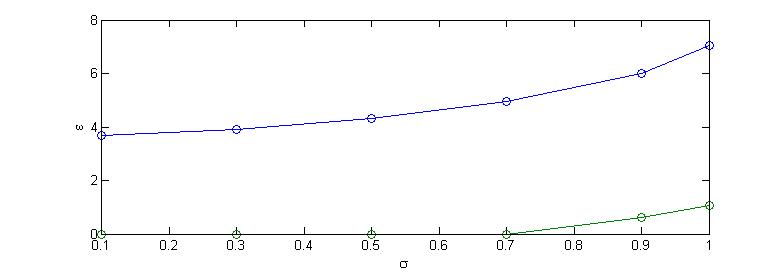
\includegraphics[width=0.9\textwidth]{figure_name.jpg}
\caption{هنا يتم إدراج وصف مختصر للشكل} \label{fig}
\end{figure}

\subsection{إدراج القوائم}
يوضح الكود التالي طريقة إدراج القوائم داخل النص. \\
يمكن تقسيم الخطأ الناتج عن العمليات الحسابية إلى خطأ القطع و خطأ التدوير. وسنشرح فيما يلي كل نوع من هذه الأخطاء:
\begin{enumerate}
\item{خطأ القطع}\\
خطأ القطع يمثل الفرق بين الحل الصحيح والحل العددي ( التقريبي) للمسألة. فمثلا، إذا كانت $f \in C^{n} [a,b] $ و $f^{n+1}$ معرفة على الفترة $[a,b]$، لذا فلأي عدد  $x \in [a,b]$  فإنه يوجد عدد $\xi(x) \in (x ,x_0)$ بحيث

\begin{equation}
f(x) = P_n(x) + R_n(x),
\end{equation}
\
بحيث أن $P_n(x)$ تسمى بكثيرة حدود تايلور من الدرجة $n$  وتعرف كمايلي
\[ P_n(x) = f(x_0)+f^{'}(x_0) ( x-x_0) + \frac{f^{''}(x_0)}{2!}( x-x_0)^2+\hdots+\frac{f^{n}(x_0)}{n!}( x-x_0)^n\]
أما $R_n (x)$ فتعرف بالباقي \eng{reminder} أو بخطأ القطع وتعرف كما يلي
\[ R_n (x) = \frac{f^{n}(\xi(x))}{(n+1)!}( x-x_0)^{n+1}\]

\begin{example}\label{eg:basics:trunc.error}
إوجد كثيرة حدود تايلور من الدرجة الثانية للدالة $f(x) = \cos(x)$ حول النقطة $x_0 = 0$، ومن ثم إستخدم كثيرة الحدود هذه من أجل تقريب قيمة $\cos(0.01)$.\\
 بما أن  $f \in C^{n} (R)$، فإنه يمكن إستخدام متسلسلة تايلور، ونظرا لأن
 \[ f(x) = \cos(x),\:  f^{'} (x) = -\sin(x), \; f^{''}(x) = -\cos(x), \: f^{'''}(x) = \sin(x),\]
 فإن
 \[ f(0) = 1,\:  f^{'} (0) = 0, \; f^{''}(0) = -1, \: f^{'''}(0) = 0,\]
 وبالتالي فإن كثيرة حدود تايلور تأخذ الشكل
 \[ \cos(x) = 1 - \frac{1}{2} x^2 + \frac{1}{6} x^3 \sin(\xi(x)); \quad \xi(x) \in (0,x). \]
\end{example}

\item{خطأ التدوير}\\
خطأ التدوير عبارة عن الفرق بين الحل العددي الذي يمكن الحصول عليه بإستخدام البيانات الأصلية والحل العددي الذي يمكن الحصول عليه بإستخدام البيانات المقربة (المدورة). وهذا النوع ينشأ عن طريقة تمثيل الأعداد في أجهزة الكمبيوتر وليس بسبب الطريقة العددية المستخدمة.
\end{enumerate}

وبشكل عام فإنه على الرغم أن كلا من خطأي القطع والتدوير يلعبان دورا هاما في دقة الحسابات العددية، إلا أن أحدهما قد يكون هو المهيمن في الحسابات العددية. فينما يهيمن خطأ التدوير في المسائل الجبرية ذات الخطوات المحدودة، فإن خطأ القطع يبرز بشكل جلي في المسائل التي تتطلب طرق تكرارية مثل التكاملات والتفاضلات.

\chapter{عنوان الفصل الثاني}
نعرف في هذا الباب طريقتين شائعتين لحساب الخطأ.

\section{مقدمة}
لحساب (أو بالأصح لتقدير) قيمة الخطأ يمكن إستخــدام إما مفهوم الخطأ  المطلق أو مفهوم الخطـأ النسبـــي. هذين النوعين يعرفان كمايلي:

\begin{align}
 \text{ القيمة التقريبية ،}ـ\--\text{ القيمة الصحيحة} = &\text{ الخطأ المطلق} \\
.     \frac{\text{الخطــأ المطلق}}{\text{ القيمة الصحيحة}}=& \text{ الخطأ النسبي}
\end{align}

\section{تطبيقات}
\begin{example}\label{eg1}
أوجد الخطأ المطلق والخطأ النسبي\cite{Beucher} في الحالات التاليـــة:
\begin{enumerate}
\item[أ -] إذا كانت القيمة الصحيحة $x = 3.141592$ والقيمة التقريبيــة $\hat{x} = 3.14$.\\
- الخطأ المطلق : $E_x \:= | x - \hat{x}| \: = 0.001592\quad $.\\
- الخطأ النسبي : $\rho_x \:= \frac{| x - \hat{x}|}{x} \: = 0.00507\quad $.
\item[ب -] إذا كانت القيمة الصحيحة $y = 1,000,000$ والقيمة التقريبيــة $\hat{y} = 999,999\quad $.\\
- الخطأ المطلق : $E_y \:= | y - \hat{y}| \: = 4\quad $.\\
- الخطأ النسبي : $\rho_y \:= \frac{| y - \hat{y}|}{y} \: = 0.000004\quad $.
\end{enumerate}
\end{example}
نلاحظ في الفقرة (أ) أنه لايوجد فرق كبير بين قيمتي الخطأ المطلق و الخطأ النسبي، لذا فإن أي منهما يمكن أن يستخدم لإختبار القيمة التقريبية لـ$x$. بينما في الفقرة (ب) فإنه على الرغم أن الخطأ المطلق كبير إلا أنه صغير مقارنة بقيمة $y$ ولذا فإنه يمكن إعتبار $\hat{y}$ تقريب جيد لقيمة $y$ لأن قيمة الخطأ النسبي صغيرة جدا. وأخيرا فإننا نلاحظ في الفقرة (ج) أنه على الرغم أن الخطأ المطلق أصغر من كلا من قيمتي $z$ و $\rho_z$ إلا أن التقريب  $\hat{z}$ هو تقريب سيء لأن قيمة الخطأ النسبي تعادل $25\%$ أي أنها قيمة كبيرة جدا.
\begin{example}\label{eg2}
الجدول التالي يوضح بعض القيم التقريبية للعدد $e = 2.7182818$ والخطأ المطلق و النسبي المقابل لكل قيمة.
\
\begin{table}[hhh!]
\centering
\begin{tabular}{|p{2.5cm}|p{2.5cm}|p{2.5cm}|}
\hline		
Approximation & Absolute Error & Relative Error \\
\hline			
$2$&$7.10^{-1}$&$2.10^{-1}$\\
$2.7$&$1.10^{-2}$& $6.10^{-3}$\\
$2.71$&$8.10^{-3}$& $3.10^{-3}$\\
$2.718$&$2.10^{-4}$& $1.10^{-4}$\\
$2.7182$&$8.10^{-5}$& $3.10^{-5}$\\
$2.71828$&$1.10^{-6}$& $6.10^{-7}$\\
\hline		
\end{tabular}

\caption{مثال  \protect \ref{eg2}}
\end{table}
\end{example}
\begin{note}\label{note 1}
 يسمى تمثيل الأعداد الذي يظهر في الجدول السابق بالتمثيل العلمي \eng{Scientific~notation}، و هو أحد الصور الشائعة لتمثيل الأعداد. 
\end{note}

\begin{note}
يقال أن العدد  $\hat{x}$  هو عدد مقرب\cite{ara1} للعدد $x$ إلى عدد $d$  من الأرقام المعنوية\footnote{عدد الأرقام المعنوية التي يحويها عدد ما مساو لعدد الأرقام التي يحتويها ذلك العدد بدءاً من أول عدد غير صفري من اليسار. فمثلا العدد $1.7320$ يحوي $5$ أرقام معنوية، فيما العدد $0.0491 $ يحوي $3$ أرقام معنوية فقط.}  \eng{Significant digits} إذا كان
\begin{equation}
\frac{|x-\hat{x}|}{x} < \frac{10^{-d}}{2},
\end{equation}
\end{note}
\begin{example}\label{eg3}
أوجد عدد الأرقام المعنوية لكل من الأعداد المقربة في مثال \ref{eg1}.\\
\begin{enumerate}
\item[أ -] إذا كانت القيمة الصحيحة $x = 3.141592$ والقيمة التقريبيــة $\hat{x} = 3.14$. فإن الخطأ النسبي $\rho_x \:= \frac{| x - \hat{x}|}{x} \: = 0.00507 < 10^{-2}/2$. وبالتالي فإن العدد $\hat{x}$ هو عدد تقريبي لـ $x$ إلى رقمين معنويين.
\item[ب -] إذا كانت القيمة الصحيحة $y = 1,000,000$ والقيمة التقريبيــة $\hat{y} = 999,999\quad $. فإن الخطأ النسبي $\rho_y \:= \frac{| y - \hat{y}|}{y} \: = 0.000004 < 10^{-5}/2$. وبالتالي فإن العدد $\hat{y}$ هو عدد تقريبي لـ $y$ إلى 5 أرقام معنوية.
\item[ج -] إذا كانت القيمة الصحيحة $z = 0.000012$ والقيمة التقريبيــة $\hat{z} = 0.000009$. فإن الخطأ النسبي $\rho_z \:= \frac{| z - \hat{z}|}{z} \: = 0.25 < 10^{0}/2$. وبالتالي فإن العدد $\hat{x}$ هو عدد تقريبي لـ $x$ بلا أرقام معنوية.
\end{enumerate}
\end{example}
\begin{excercise}
كم عدد الأرقام المعنوية بين العدد $x = 0.9949$  و $\hat{x}=0.9951$؟
\end{excercise} 

\section{نص إنجليزي}
\eng{For any academic/research writing, incorporating references into a document is an important task. Fortunately, LaTeX has a variety of features that make dealing with references much simpler, including built-in support for citing references. However, a much more powerful and flexible solution is achieved thanks to an auxiliary tool called BibTeX (which comes bundled as standard with LaTeX). Recently, BibTeX has been succeeded by BibLaTeX, a tool configurable within LaTeX syntax.}

\addcontentsline{toc}{section}{المراجع}
\bibliographystyle{unsrt}
\bibliography{المراجع}{}
\begin{thebibliography}{10}
\selectlanguage{english}
\bibitem{Beucher}
O. Beucher and M. Weeks, 
\newblock Introduction to MATLAB \& Simulink: A Project Approach,
\newblock Cambridge Press, 
\newblock 2015.
\bibitem{Downey}
A. Downey, 
\newblock Physical Modeling in MATLAB,
\newblock UOM Press,
\newblock 2016.
\bibitem{Attaway}
S. Attaway, 
\newblock Matlab: A Practical Introduction to Programming and Problem Solving,
\newblock XYZ Press,
\newblock 2010.
\selectlanguage{arabic}
\bibitem{ara1}
م. الحامد
\newblock عنوان الكتاب، دار النشر، 2017
\end{thebibliography}

\end{document} 
